\section{Entwicklung} % (fold)
\label{sec:entwicklung}
	Dieses Kapitel soll den Entwicklungsprozess konkretisieren und den Optimierungsprozess einer Webanwendung aufzeigen. Es soll erläutern, welche Fragen sich stellten und welche Antworten darauf gefunden wurden. Wie bestimmte Probleme gelöst wurden. Welche Tools und Hilfsmittel zur verwendung kamen. Dies soll ein Bewusstsein dafür schaffen, was möglich ist und wie eine technische Umsetzung aussehen kann. 
	
	\subsection{Tools}
	\label{sub:tools}
		Dies ist eine Auflistung an Tools und nützlichen Seiten, die entweder im Projekt verwendung fanden, oder die für Wertvoll befunden wurden und deshalb hier ihren Platz finden, damit jeder für sich entscheiden kann, ob der Einsatz davon sinnvoll sein könnte.

		\subsubsection{Google Chrome Developer Tool} % (fold)
		\label{ssub:google_chrome_developertool}
			Dieses Tool ist über die Taste F12 im Chrome Browser zu finden. Nützliche Features sind: 

			\begin{itemize}
				\item \texttt{Device Emulation} \footnote{Bei geöffnetem Tool (F12): strg + shift + M oder klick auf das Smartphone Symbol}: Damit lassen sich verschiedene Devices wie Smartphones, Ipad oder verschiedene Desktopauflösungen simulieren. Auch das Touch verhalten wird Simuliert.
				\item In der Device Emulation lässt sich auch die Netzwerkgeschwindigkeit simulieren. Dies ist allerdings nur eine Simulation und kann unter wahren Bedingungen stark abweichen.
				\item Netzwerk: Hier lässt sich das Wasserfallmodell nachvollziehen. Auch lässt sich hier das Caching des Browsers abschalten, wärend das Developer Tool geöffnet ist.
				\item Audits: Unter diesem Reiter bekommt man erste Informationen, welche Verbesserungen es für diese Seite aus dem Gesichtspunkt der Performance ergeben. So wird zum Beispiel aufgezeigt, wie viele CSS Selektoren auf dieser Seite gar keine verwendung finden (gerade bei CSS-Frameworks wie Bootstrap kann es sein, dass rund 90\% der Selektoren keine Verwendung haben)
			\end{itemize}
		% subsubsection google_chrome_developertool (end)

		\subsubsection{Google Pagespeed Insight} % (fold)
		\label{ssub:google_pagespeed_insight}
			Pagespeed Insight ist ein Analysetool für Webanwendungen. Per URL Eingabe wird die Anwendung Aufgerufen und gegen die "`Best Practices"' von Google getestet: \footnote{ \url{http://tinyurl.com/nvxksks} }. Dabei wird ein Rating von 1 (schlecht) bis 100 (gut) vergeben. Mobile und Desktop Version werden voneinander unabhängig bewertet. Findet das Tool verstöße gegen die \texttt{best practices}, so gibt es Hilfestellungen wie zum Beispiel weiterführende Links oder Hinweise zur Behebung des Problems. Für die Verbesserung der Perfomance ist dieses Tool eines der besten Anlaufziele, um einen Überblick zu bekommen wo sich die Probleme befinden. Pagespeed Insight gibt es auch als Plugin für das Google Chrome Developer Tool.\footnote{Plugin - Pagespeed Insight: \url{http://tinyurl.com/mv8fcx8}}
		
		% subsubsection google_pagespeed_insight (end)

		\subsubsection{Google Closure Compiler} % (fold)
		\label{ssub:closure_compiler}
			Ein simples Tool von Google\footnote{\url{http://closure-compiler.appspot.com/}}, mit der Aufgabe Javascript zu verkleinern. Dieser Vorgang nennt sich auch "`minify"' und ist auch für HTML und CSS möglich. Ein Beispiel:

			\begin{lstlisting}[captionpos=t, caption=Input, label=lst:minifyInput]
			/**
			 * urlEncodes an object to send it via post
			 * @param  {Object} object Object with key value pairs
			 * @return {String}        string in format key=value&foo=bar
			 */
			var urlEncode = function (object) {
			  var encodedString = '';
			  for (var prop in object) {
			    if (object.hasOwnProperty(prop)) {
			      if (encodedString.length > 0) {
			          encodedString += '&';
			      }
			      encodedString += encodeURI(prop + '=' + object[prop]);
			    }
			  }
			  return encodedString;
			};
			\end{lstlisting}

			Wird zu:

			\begin{lstlisting}[captionpos=t, caption=Output, label=lst:minifyOutput, breaklines=false]
			var urlEncode=function(c){var a="",b;for(b in c)c.hasOwnProperty(b)&&
			(0<a.length&&(a+="&"),a+=encodeURI(b+"="+c[b]));return a};
			\end{lstlisting}
		
		% subsubsection closure_compiler (end)

		\subsubsection{Webpagetest} % (fold)
		\label{ssub:webpagetest}
			\url{Webpagetest.org} ist das wohl umfangreichst und beste Website-Analysetool welches im Internet zu finden ist. Es ist ein kostenloser Service der hauptsächlich von Patrick Meenan entwickelt wurde. Das Tool ist leicht zu bedienen aber schwer zu beherschen ("`easy to use, hard to master"') und es gibt zahllose Einstellungen und undokumentierte Funktionen auf die man nur in Vorträgen oder Foren stoßt. Es gibt auch ein Buch, welches sich nur mit diesem Tool beschäftigt, beim Verlag \texttt{O'Reilly}.\footnote{Buch \url{http://shop.oreilly.com/product/0636920033592.do}}.	Die Features für Webpagetest sind vielseitig:

			\begin{itemize}
				\item Es lassen sich Webanwendungen mittels eines in der realität existierenden Geräts testen. So kann vom Standort Dulles VA ein MOTOG zum Testen einer Seite verwendet werden. Dieses Gerät ruft dann auch wirklich die eingegebene URL auf und die darunterliegende Schicht misst die Zeit. Abbildung \ref{fig:wpt-android} zeigt den Teststandort Dulles VA.\footnote{Einen detailierten einblick vom Gründervater und Entwickler Patrick Meenan gibt es hier: \url{http://tinyurl.com/o4b3rxh}}

				\begin{figure}[htbp]
					\begin{center}
						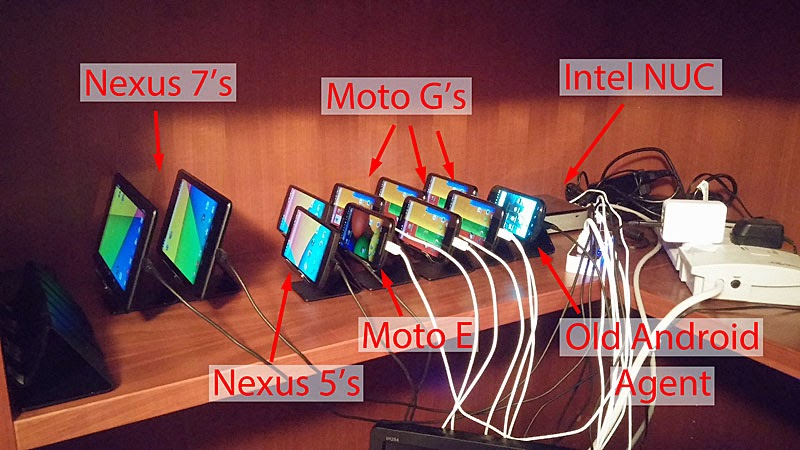
\includegraphics[width=0.5\textwidth]{wpt-android.jpg}
						\caption{Webpagtest Android device farm (Abbildung von \autocite{meenan15})}
						\label{fig:wpt-android}
					\end{center}
				\end{figure}
				\item Webpagetest hat die wohl genauste Erfassung von Netzwerkzeiten und spiegelt damit realitätsgetreu die Ladezeiten einer Seite wieder.

				\item Webpagtest liefer eine enormes Spektrum an Daten und Diagrammen, was ausführliche Analysen zulässt.

				\item Speed Index: Dies ist eine von diesem Tool eigene Maßeinheit zum bestimmen der \texttt{Perceived Performance} einer Seite.

				\begin{quote}
					\textit{"`'The Speed Index metric was added to WebPagetest in April, 2012 and measures how quickly the page contents are visually populated (where lower numbers are better).  It is particularly useful for comparing experiences of pages against each other (before/after optimizing, my site vs competitor, etc) and should be used in combination with the other metrics (load time, start render, etc) to better understand a site's performance."'}\autocite{wegpagetestDocs}
				\end{quote}

				\item Man kann Tests direkt miteinander vergleichen. Das ist möglich, indem diese URL eingegeben wird: \url{www.webpagetest.org/video/compare.php?tests=} und nach dem "`="' Zeichen die Test ID eingibt, beispielsweise "`150310\_8E\_GRH"'.
				Mit einem Komma getrennt wird eine 2. oder 3. ID angefügt. Die Tests werden dann in einer Vergleichsansicht dargestellt.

				\item Filmstrip Ansicht: Damit lässt sich visuell erkennen, wann welches Element gerendet wird.

				\item Video erstellung: Aus der Filmstrip Ansicht lässt sich ein Video erstellen. Das ist vor allem interessant, wenn mit der Vergleichsmethode mehrere Tests geladen sind. Der Ladevorgang der Testläufe wird dann in einem Video Parallel abgespielt. Vor allem für Präsentationen oder vorher / nachher Vergleiche ist dies nützlich.

				\item Test History: Durch eine Registrierung auf der Seite wird ein eigenes Testprofil angelegt in dem alle Test-ID's gespeichert werden.

				\item API: Webpagtest hat eine offene API (Schnittstelle) durch die das Tool von außerhalb erreichbar ist. So lässt sich ein Test beispielsweise in Google-Spreadsheets aufrufen und das Ergebnis direkt in eine Tabelle schreiben. Mehr dazu in Punkt: \ref{..} ?. %todo

			\end{itemize}
		% subsubsection webpagetest (end)	

		\subsubsection{Pingdom} % (fold)
		\label{ssub:pingdom}
			Tests wie Webpagtest nur ungenauer :D
			Monitoring feature

		
		% subsubsection pingdom (end)

		\subsubsection{Speedcurve} % (fold)
		\label{ssub:speedcurve}
			frontend monitoring
			Vergleicht zur Konkurrenz
		% subsubsection speedcurve (end)

		\subsubsection{Google Spreadsheet} % (fold)
		\label{ssub:google_spreadsheet}
			Script Schnittstelle
			Bulk Webpagetest
			Link zu Daten geben
		
		% subsubsection google_spreadsheet (end)

		\subsubsection{Feed the Bot} % (fold)
		\label{ssub:feed_the_bot}
			Best practices
				
		% subsubsection feed_the_bot (end)

		\subsubsection{Critical Path CSS Generator} % (fold)
		\label{ssub:critical_path_css_generator}
		
		% subsubsection critical_path_css_generator (end)

		\subsubsection{moz Jpeg} % (fold)
		\label{ssub:moz_jpeg}
		
		% subsubsection moz_jpeg (end)

		\subsubsection{Http Archive \& bigqueri.es} % (fold)
		\label{ssub:http_archive_bigqueri_es}
			
		% subsubsection http_archive_bigqueri_es (end)

		\subsubsection{Perf Tooling Today} % (fold)
		\label{ssub:perf_tooling_today}
		
		% subsubsection perf_tooling_today (end)

		\subsubsection{Twitter} % (fold)
		\label{ssub:twitter}
		
		% subsubsection twitter (end)



	% subsection tools (end)


	\subsection{Ausgangspunkt}
	\label{sub:ausgangspunkt}
	
	% subsection ausgangspunkt (end)

	\subsection{Prozess der Validierung}
	\label{sub:prozess_der_validierung}
	
	% subsection prozess_der_validierung (end)

	

% section entwicklung (end)